\documentclass[10pt,twocolumn,letterpaper]{article}

\usepackage{cvpr}
\usepackage{times}
\usepackage{epsfig}
\usepackage{graphicx}
\usepackage{amsmath}
\usepackage{amssymb}
\usepackage{url}
\usepackage{subfigure}
\usepackage[utf8]{inputenc} %'표시
\usepackage{parskip}
\usepackage{caption}
\usepackage{rotating}
\usepackage{hvfloat}

% Include other packages here, before hyperref.

% If you comment hyperref and then uncomment it, you should delete
% egpaper.aux before re-running latex.  (Or just hit 'q' on the first latex
% run, let it finish, and you should be clear).
\usepackage[pagebackref=true,breaklinks=true,letterpaper=true,colorlinks,bookmarks=false]{hyperref}

% \cvprfinalcopy % *** Uncomment this line for the final submission

\def\cvprPaperID{****} % *** Enter the CVPR Paper ID here
\def\httilde{\mbox{\tt\raisebox{-.5ex}{\symbol{126}}}}

% Pages are numbered in submission mode, and unnumbered in camera-ready
\ifcvprfinal\pagestyle{empty}\fi
\begin{document}

%%%%%%%%% TITLE
\title{Reconstructing an axially symmetric transparent object using a single-view image}

\author{First Author\\
Institution1\\
Institution1 address\\
{\tt\small firstauthor@i1.org}
% For a paper whose authors are all at the same institution,
% omit the following lines up until the closing ``}''.
% Additional authors and addresses can be added with ``\and'',
% just like the second author.
% To save space, use either the email address or home page, not both
\and
Second Author\\
Institution2\\
First line of institution2 address\\
{\tt\small secondauthor@i2.org}
}

\maketitle
%\thispagestyle{empty}

%%%%%%%%% ABSTRACT
\begin{abstract}
   This paper proposes a novel method to estimate the inner shape of a transparent object based on the deflection of visible rays. Our ray tracing approach on deflection sequentially estimates the refractive index and the inner shape of a transparent object and furthermore the refractive index of liquid in it. As a practical application, it is demonstrated to realistically render a wine glass with various kinds of liquid.
\end{abstract}

%%%%%%%%% BODY TEXT
\section{Introduction}

Accurate modeling and rendering of a transparent object has been a challenging problem in Computer Graphics. Generally, the problem incorporates the estimation of optical properties as well as geometrical estimation for a target object. To realistically visualize translucency, refractive index and absorption coefficient are key elements taken into account through the modeling and rendering process. Although their values are known for specific materials, they are not usually provided for daily items, such as wine glasses, targeted in environmental modeling and rendering. Even those items tend to be manufactured by compounding different kinds of materials, which makes it impossible to retrieve the exact optical properties of a composite object from a known database. This paper presents a method to accurately estimate a refractive index of a thin transparent object based on the deflection measurement of propagating rays. 
On the other hand, there is a challenging matter in the geometrical estimation of a transparent object, which is the inner shape. Unlike the outer shape of an object which can be straightforwardly measured by vision sensors, inner shapes are generally intractable in acquiring direct information on geometry. X-ray has been widely adopted for revealing inner geometry especially in a medical and a security domain. Although it has a strength to relate the absorbance of an object to its inner shape, its usability is limited by safety matters. Also, that characteristics is not applicable to a thin object where the absorbance is negligible. Therefore, this paper proposes a novel method to estimate the inner shape of a transparent object based on the deflection of visible rays. Our ray tracing approach on deflection sequentially estimates the refractive index and the inner shape of a transparent object and furthermore the refractive index of liquid in it. As a practical application, it is demonstrated to realistically render a wine glass with various kinds of liquid.

%-------------------------------------------------------------------------
\section{Related Work}

Volumetric reconstruction of transparent objects is a challenging inverse problem, 
known from optics \cite{vest1985}. With development of computer graphics the demand in 
$3D$ scanning of transparent objects brought this problem to a new level of interest.
Several publications on this topic appeared proposing different solutions. For example, in~\cite{Kutulakos:2005:ICCV} the shape of the glass object was estimated using direct ray measurements, but the shapes there are limited to maximum of two interfaces in total which means that the suitable to reconstruction shapes variations are very limited. Another approach is based on immersing the object into the special liquid. It can be the liquid with similar refractive index, such that the rays, when passing through such combined volume are propagating almost straight. Then a standart tomography approach can be used to recover the volume~\cite{Trifonov:2006:TRT}. Or, another example, is immersing into fluorescent liquid, as was done by ~\cite{Hullin08:FIRS}. Unfortunately, these approaches requires to die the object into a special solutions, which is sometimes not desirable. In optics there was attempt to recover axially-symmetric objects~\cite{Maruyama:77}, but it was limited by complicated optical setup, which is not easy to expand for larger objects (like glasses) and the method proved to work only for materials with relatively small refractive index difference between the object and surrounding medium. A detailed overview of the area can be found in the following state of the art report,~\cite{Ihrke10:TSOR}.

\section{Estimation of Refractive Index}

This section introduces our computational method for accurately estimating refractive index of an object. We assume that the target object is rotationally symmetry and the refractive index is constant for the entire volume of it. The first step of our method was locating two-interface regions over the obtained deflection map. A flip image as shown in Figure~\ref{flip} (a) was used to tell the number of interfaces at the reference view. When such a two-colored light in red and green is illuminated to the object, the colored pattern inside of the object changes according to the number of interfaces. For example, in the blue dotted region of the figure, the colored pattern was reversed from one in background. This means that the number of interface in the region is two or six. The yellow dotted region with the same pattern with the background can be interpreted as four or eight interfaces. For a simple object, the blue and yellow regions correspond to two and four interfaces.

\begin{figure}
  \centering
	\subfigure[flip image]{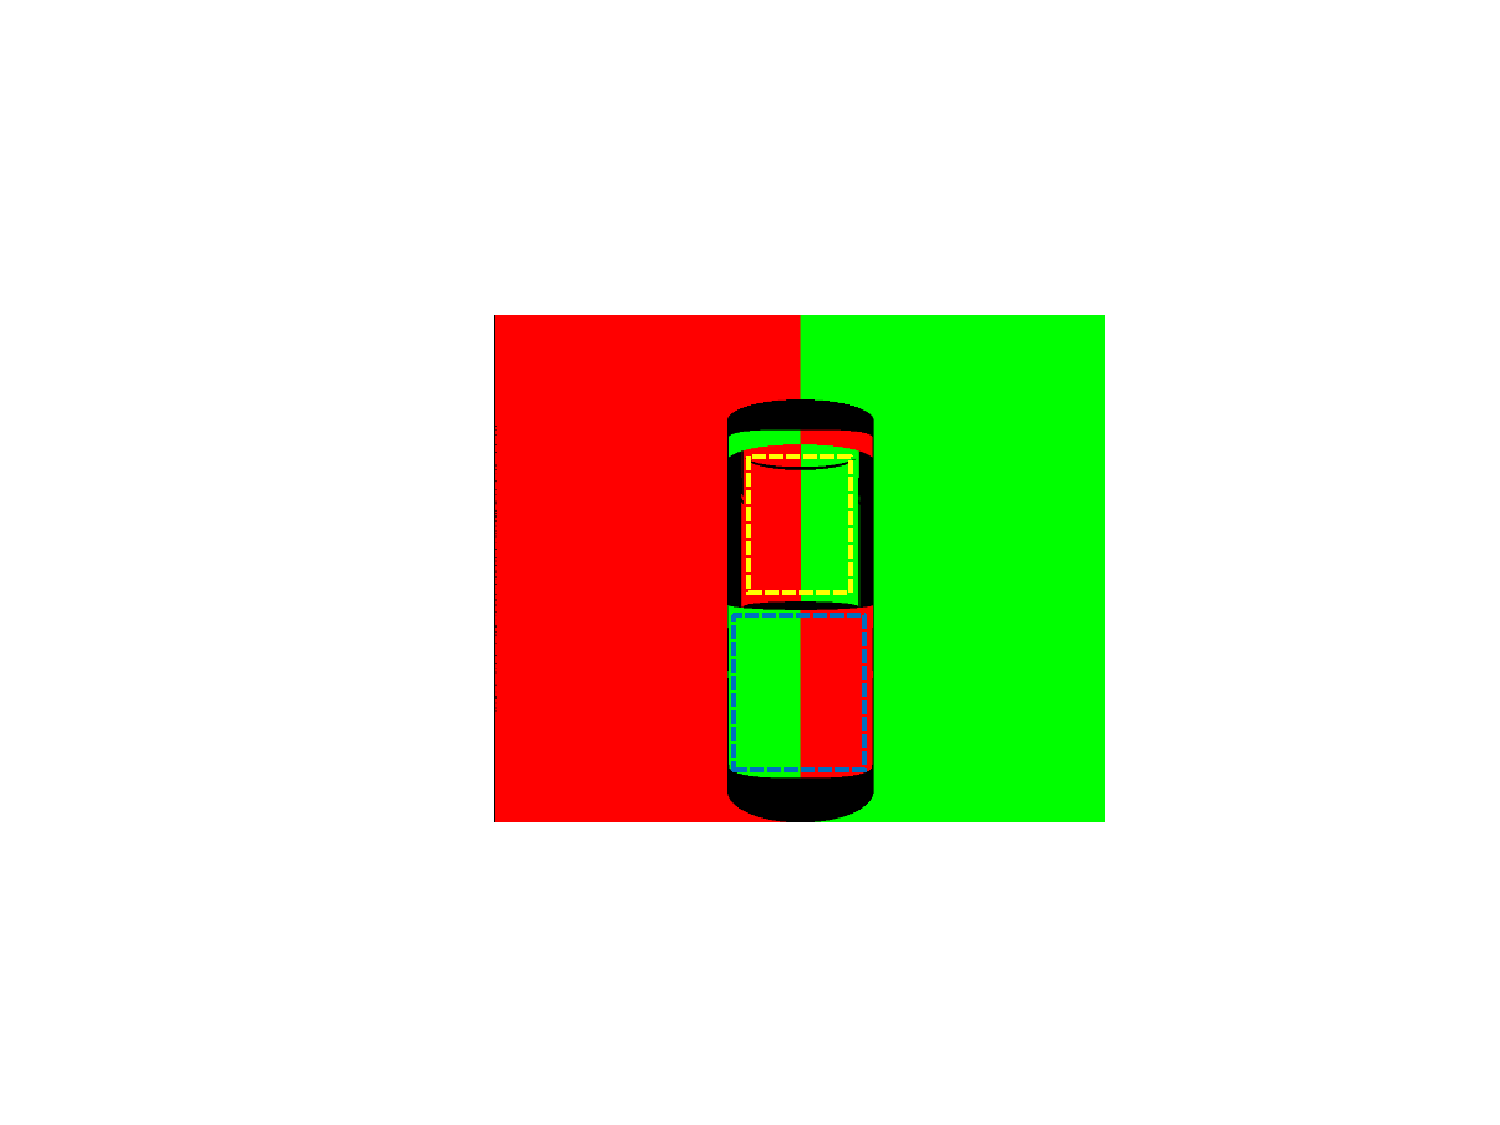
\includegraphics[width=0.48\linewidth]{figure/flip1.pdf}}
	\subfigure[error map]{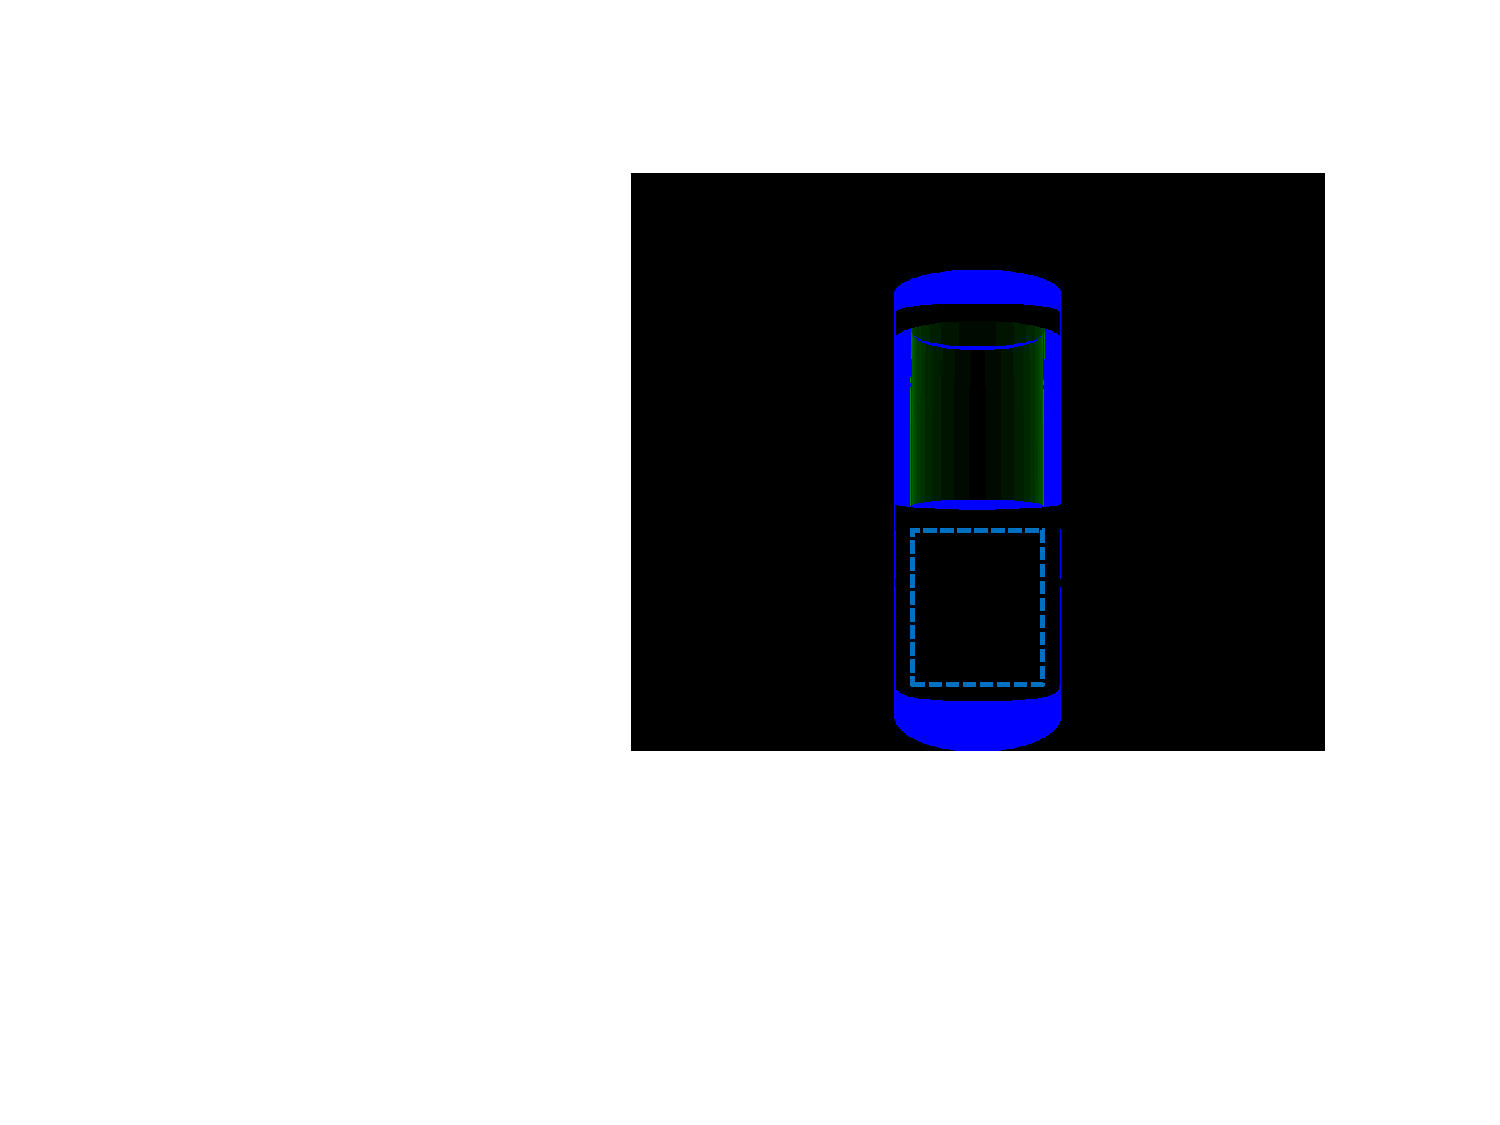
\includegraphics[width=0.48\linewidth]{figure/emap1.pdf}}		
  %\vspace{-5ex}
  \caption{(a) shows an example of a flip image for identifying the number of interfaces. A positional error map (b) is generated by visualizing positional error values between computationally traced and measured rays where the brighter green color indicates the higher error.}
  \label{flip}
  %\vspace{-2ex}
\end{figure}

As a next step, ray tracing was performed in the two-interface region to accurately estimate the refractive index. As iteratively updating the index from an initial guess, a positional error map between computationally traced and measured rays was generated for each index as shown in Figure~\ref{flip} (b). The accurate refractive index, 1.5 in our experimental data (Figure~\ref{graph}), was retrieved by searching for minimized sum of error in the blue dotted region.

\begin{figure}
  \centering
	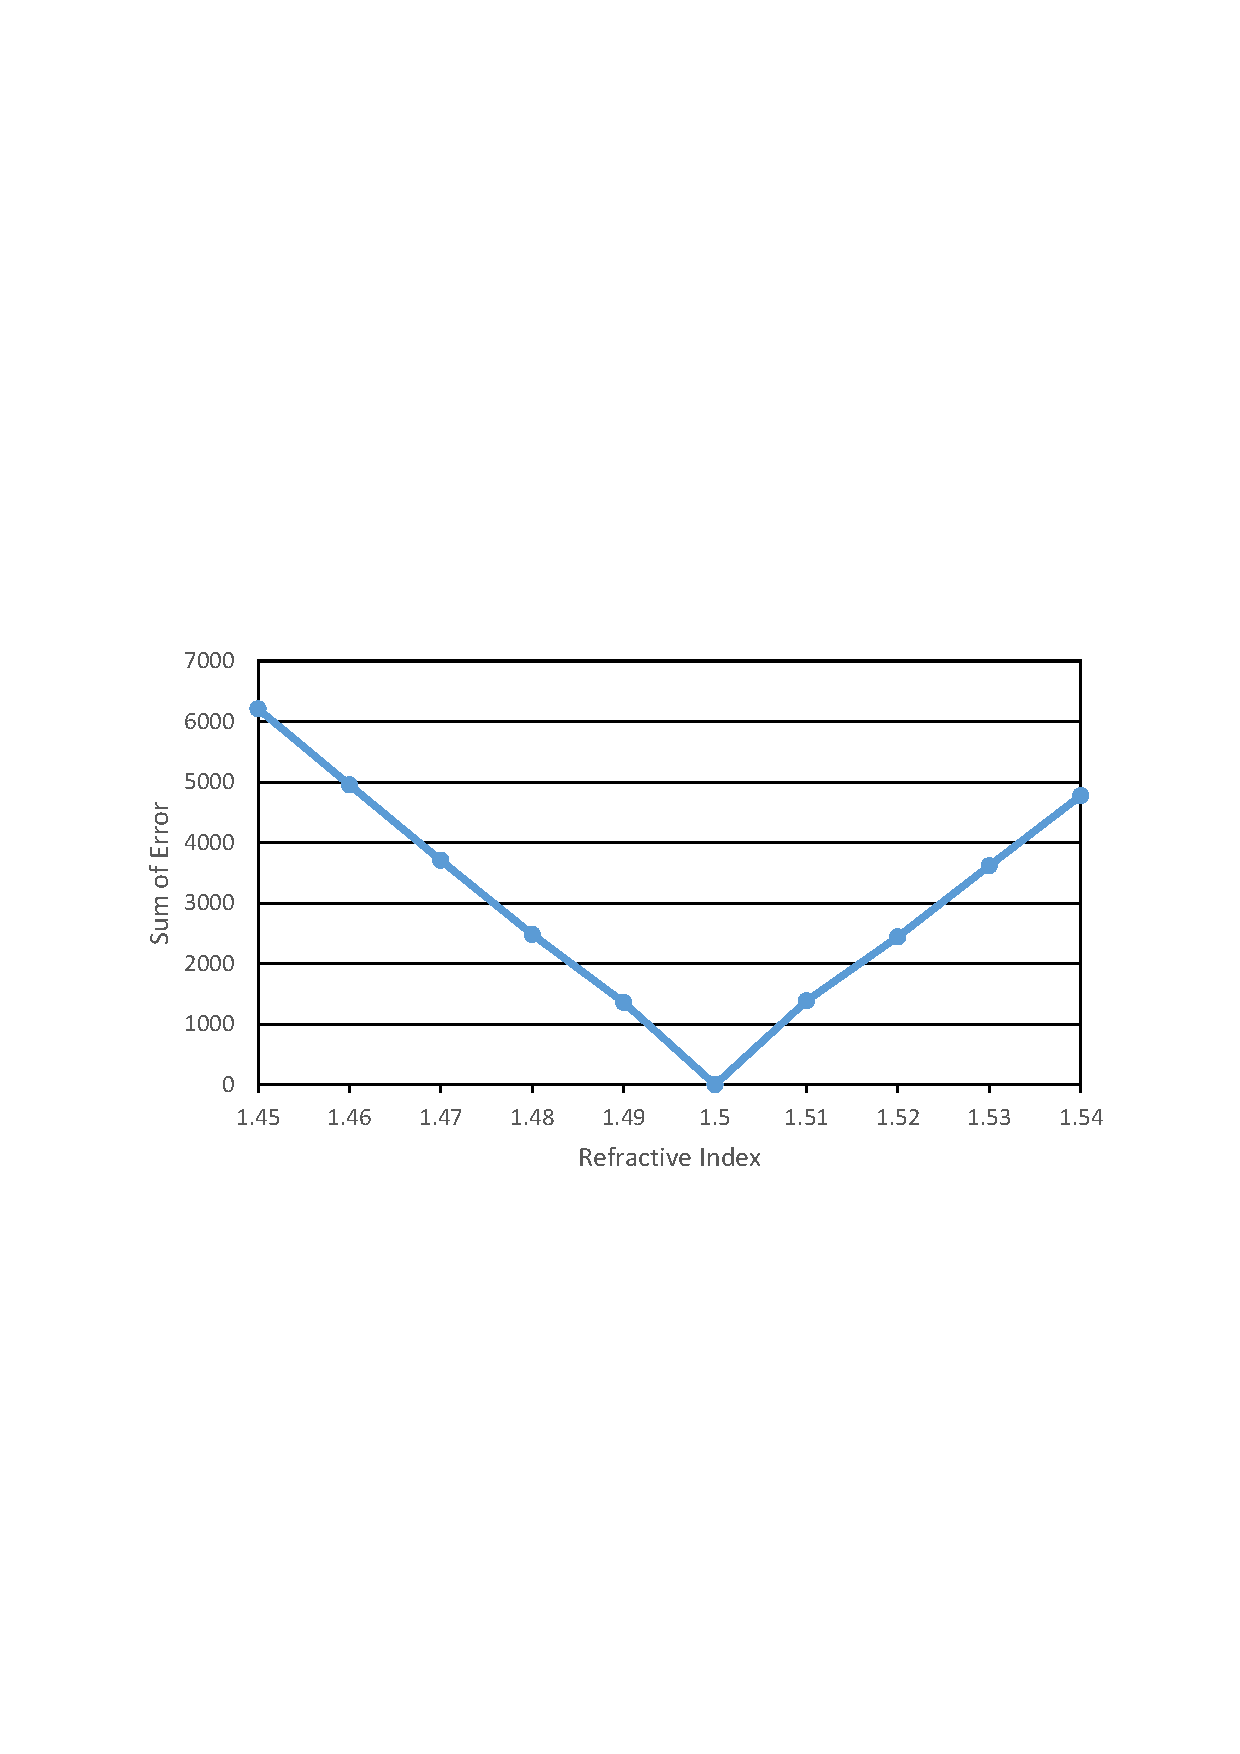
\includegraphics[width=1\linewidth]{figure/Ref_graph3.pdf}	
  %\vspace{-5ex}
  \caption{Sum of positional errors in the blue dotted region in Figure~\ref{flip} (b) according to variation in refractive index.}
  \label{graph}
  %\vspace{-2ex}
\end{figure}

\section{Estimation of Inner Geometry}
This section describes our computational method to estimate the inner geometry of a transparent object based on refractions in ray tracing. Inner geometry is defined as the geometrical information of surfaces enclosed by outer surfaces as shown in Figure~\ref{ray_dia}. By the definition, only four-interface regions for the object given in Section 2 are considered for our computation. A two-interface region is considered as a solid region without any internal structure, which is not a target of the method in this section. As illustrated by the conceptual ray diagram, our computational method estimates the unknown inner geometry, t1 and t2, in the manner of minimizing the sum of positional errors between traced rays and measurements. Here is described our computational algorithm in detail, which targets an object in rotational symmetry for simplicity. 
The first step was a coarse estimation of inner geometry from a 2D image. From the projected 2D silhouette in Figure~\ref{coarse}, the geometry of inner surfaces was obtained by segmenting the four regions corresponding to inner and outer surfaces. Then, the coarse inner geometry was used as an input for a refinement process based on ray tracing. At each cross-section, the control parameter, t1, was refined by searching for the value to satisfy the condition where sum of positional errors between traced rays and measurements. For the ray tracing, outer geometry was predetermined and the traveling distance, t2, between the third and fourth interfaces was given from the latest refinement of inner geometry. By iterating this process until the change of errors was smaller than a threshold, the accurate inner geometry was acquired. Figure~\ref{cand} demonstrates refined inner shapes in upper row and corresponding error maps marked with green pixels in bottom row. Figure~\ref{render} is the final rendering for the model of the given object. Note that the inner geometry is accurately visualized in the figure. 

\section{Results}


\begin{figure}
  \centering
	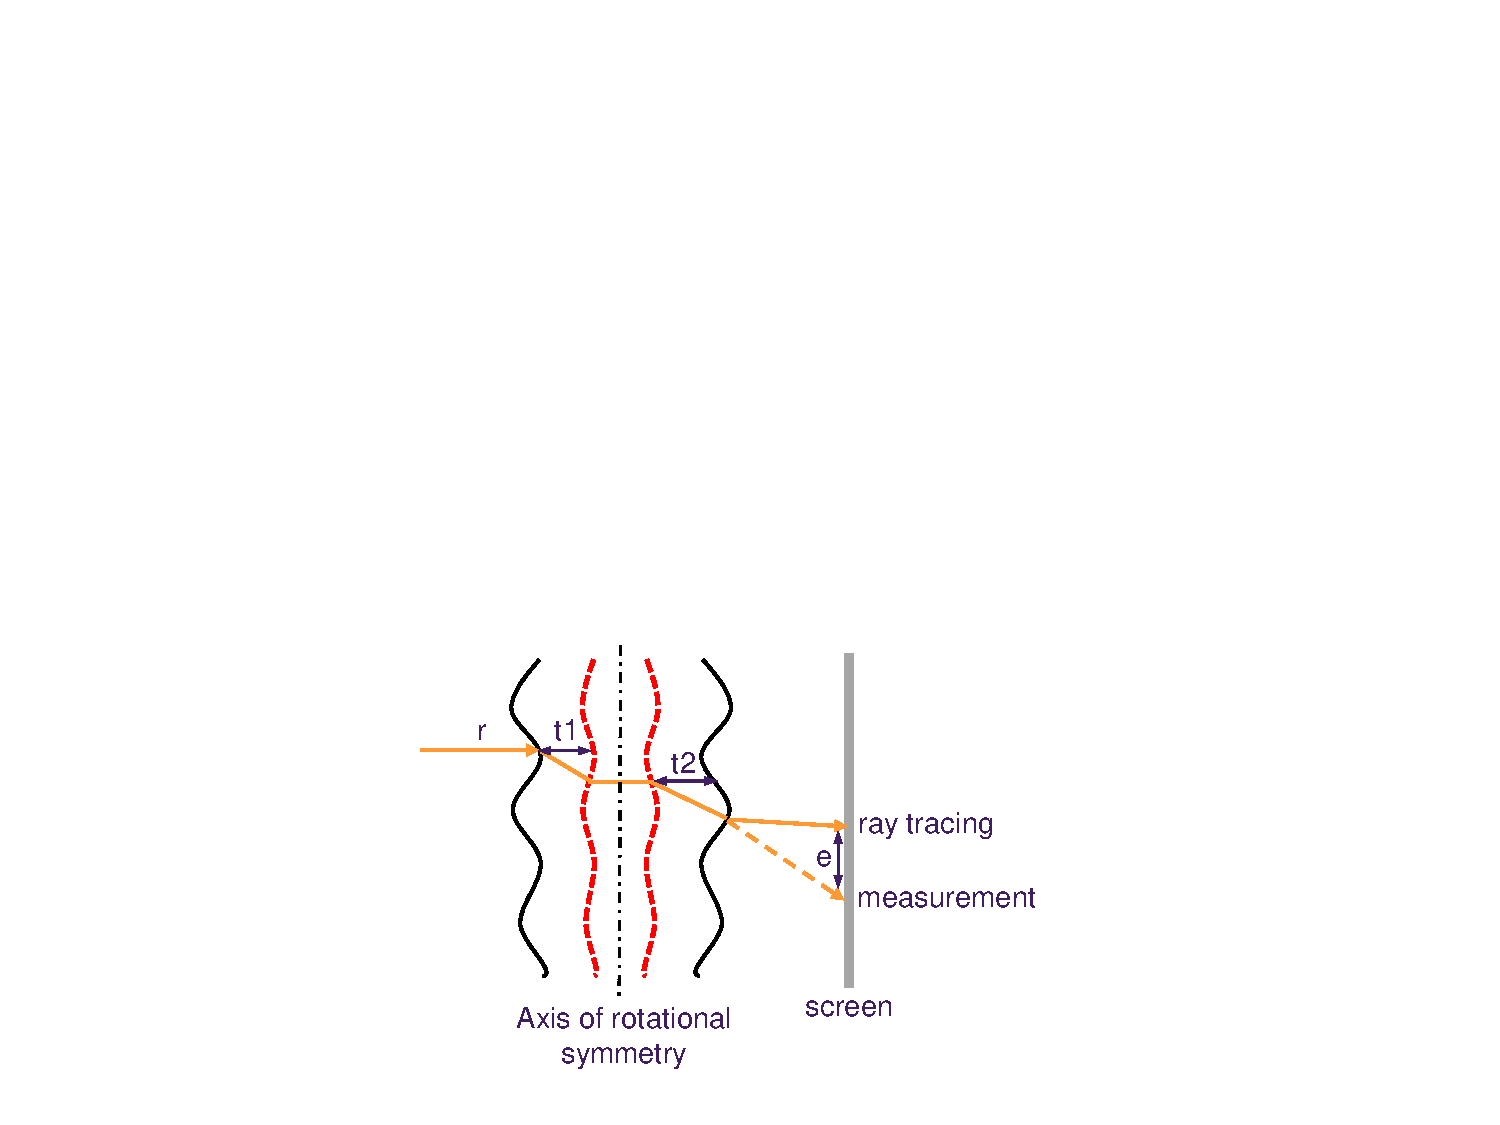
\includegraphics[width=1\linewidth]{figure/ray_dia1.pdf}	
  %\vspace{-5ex}
  \caption{A diagram of a ray traveling through four interfaces. The unknown inner geometry, t1 and t2, is estimated by minimizing the sum of positional errors, e, between ray tracing and measurement.}
  \label{ray_dia}
  %\vspace{-2ex}
\end{figure}

The accuracy of our reconstruction algorithm was tested using simulated data first, see Section~\ref{sec:our_approach}.

Our experimental setup consists of a machine vision camera and an LCD display, see [{\bf{add setup picture}}]. We place the object
in front of the screen close to its surface in order to minimize deflections in the central part of the object. This position
also allows to keep the screen and the object both in focus. The data acquisition process consist of sequential capturing images of the scene for each vertical and horizontal line displayed on the screen. To calibrate initial rays positions on the screen the
same sequence of capturing is then repeated, but without the object. Finally, to calibrate the position of the screen we are taking an image of the checkerboard displayed on the screen. The camera's pose and intrinsics calibration and the screen position estimation was done using Bouguet’s calibration toolbox~\cite{CalibToolbox}.

We estimated the outer silhouette of the object using the captured images and the fact, that there is a light distortion on the
object's border, see Figure [fig.]. The initial symmetry axis of the object was estimated using the position of the screen, the distance of the center of the object from the screen and the projected on the camera image axis of symmetry of the silhouette of the object. Using acquired images of the object backlighted with different vertical and horizontal lines we then estimated the rays deflection map, see Figure [fig.]. Any pair of vertical and horizontal lines provide us with a single common pixel, which $3D$ position on the screen was computed from its $2D$ position on the camera image by projecting corresponding camera ray on the screen plane. The deflected pixel on the camera image was computed as the brightest common pixel of the corresponding vertical and horizontal images.

\begin{figure}
  \centering
	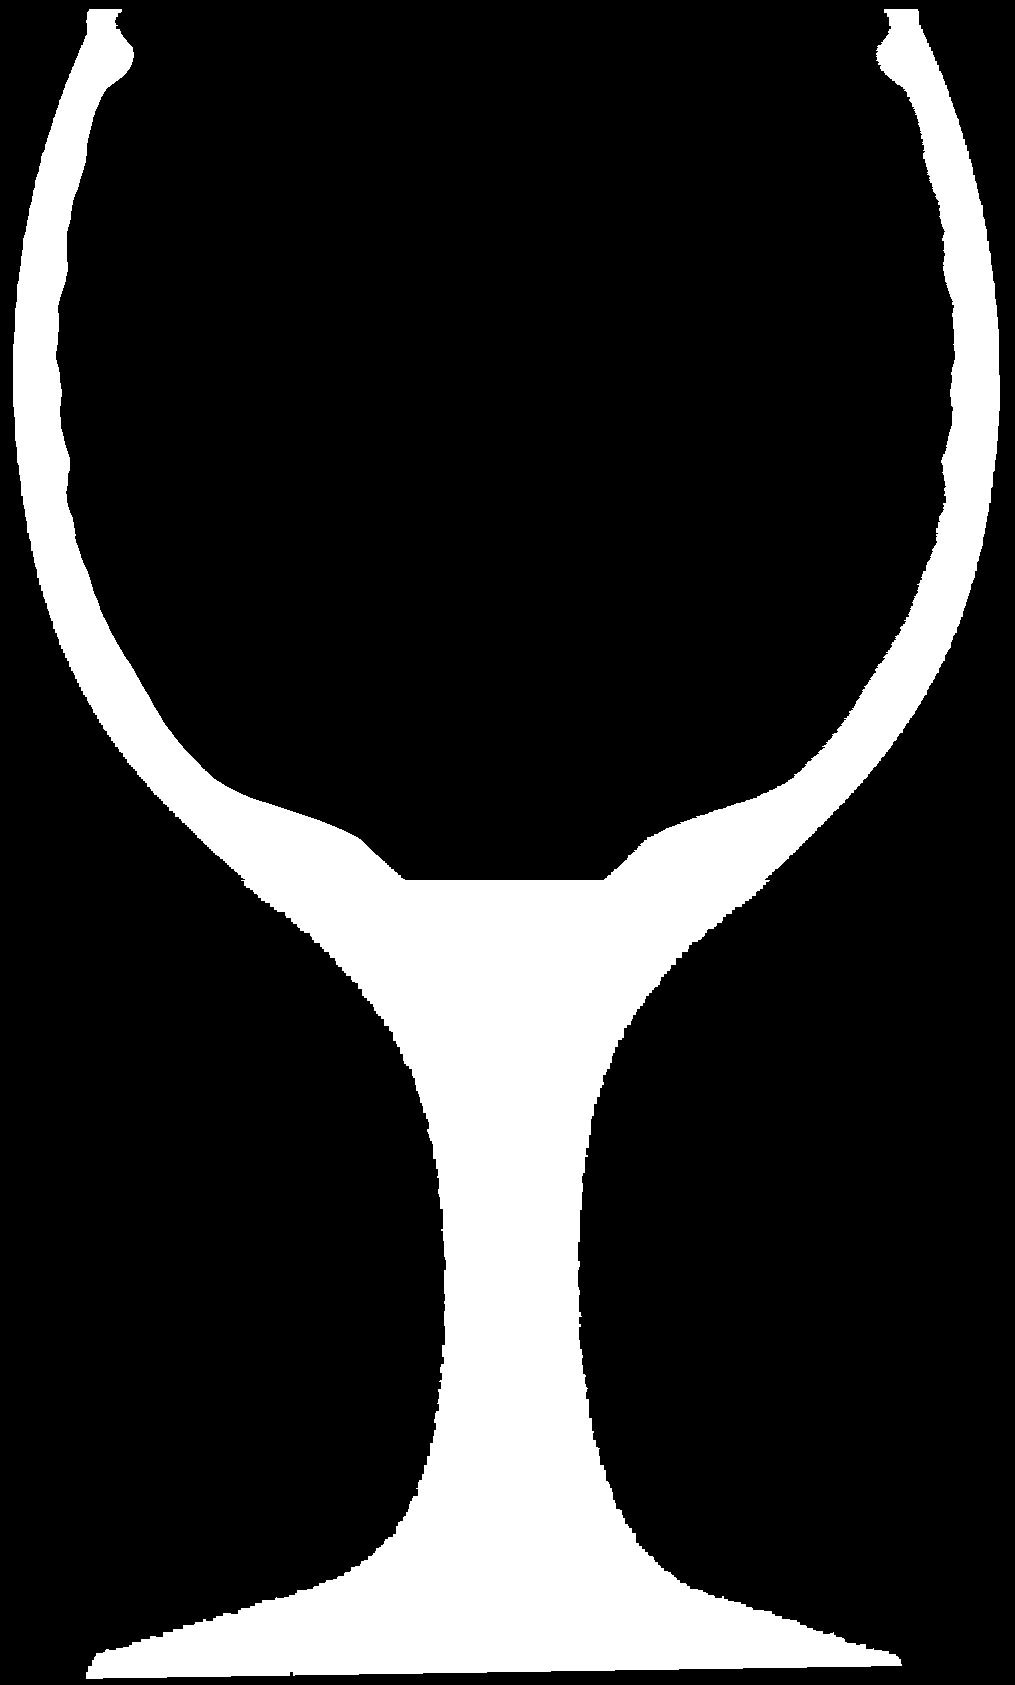
\includegraphics[height=0.7\linewidth]{figure/coarse.jpg}	
  %\vspace{-5ex}
  \caption{A 2D image to be used for the initial estimation of inner geometry.}
  \label{coarse}
  %\vspace{-2ex}
\end{figure}

Using estimated above axis of symmetry and deflection map we produced a flip image, Figure [figure], necessary for the reconstruction algorithm. The colour of each pixel on the flip image was selected as red (green) if the corresponding to that pixel camera ray is crossing the screen from the left (right) side of the projected (using the camera projection center) on the screen axis of symmetry.  

The initial inner silhouette of the object was estimated from intensity image, estimated from polarization measurements[?] and
using our recently computed flip image. [fig.].

We used outer silhouette of the object and the fact, that the object is close to axially-symmetric to compute the outer shape
initial estimation. We did that by calculating the radius of the object at each point on the symmetry axis using raytracing of the border of the silhouette image and knowing the $3D$ position of the axis. In a similar fashion we estimated inner shape of the object from the inner silhouette.

Having our deflection map and initial object's shape estimation projected onto $2D$ plane spanned by the camera centre and the
axis of symmetry, we then estimated a refined object's shape using our $2D$ surface optimization algorithm, described above [{\bf{to do: describe it above}}]. 

This refined version of the object's shape then was used as initial guess by our final $3D$ reconstruction algorithm [{\bf{reference
to the previous section}}].

%\begin{figure*}[t]
  %\centering
  %\mbox{} \hfill \vfill   
  %\subfigure[Candidates of inner geometry]{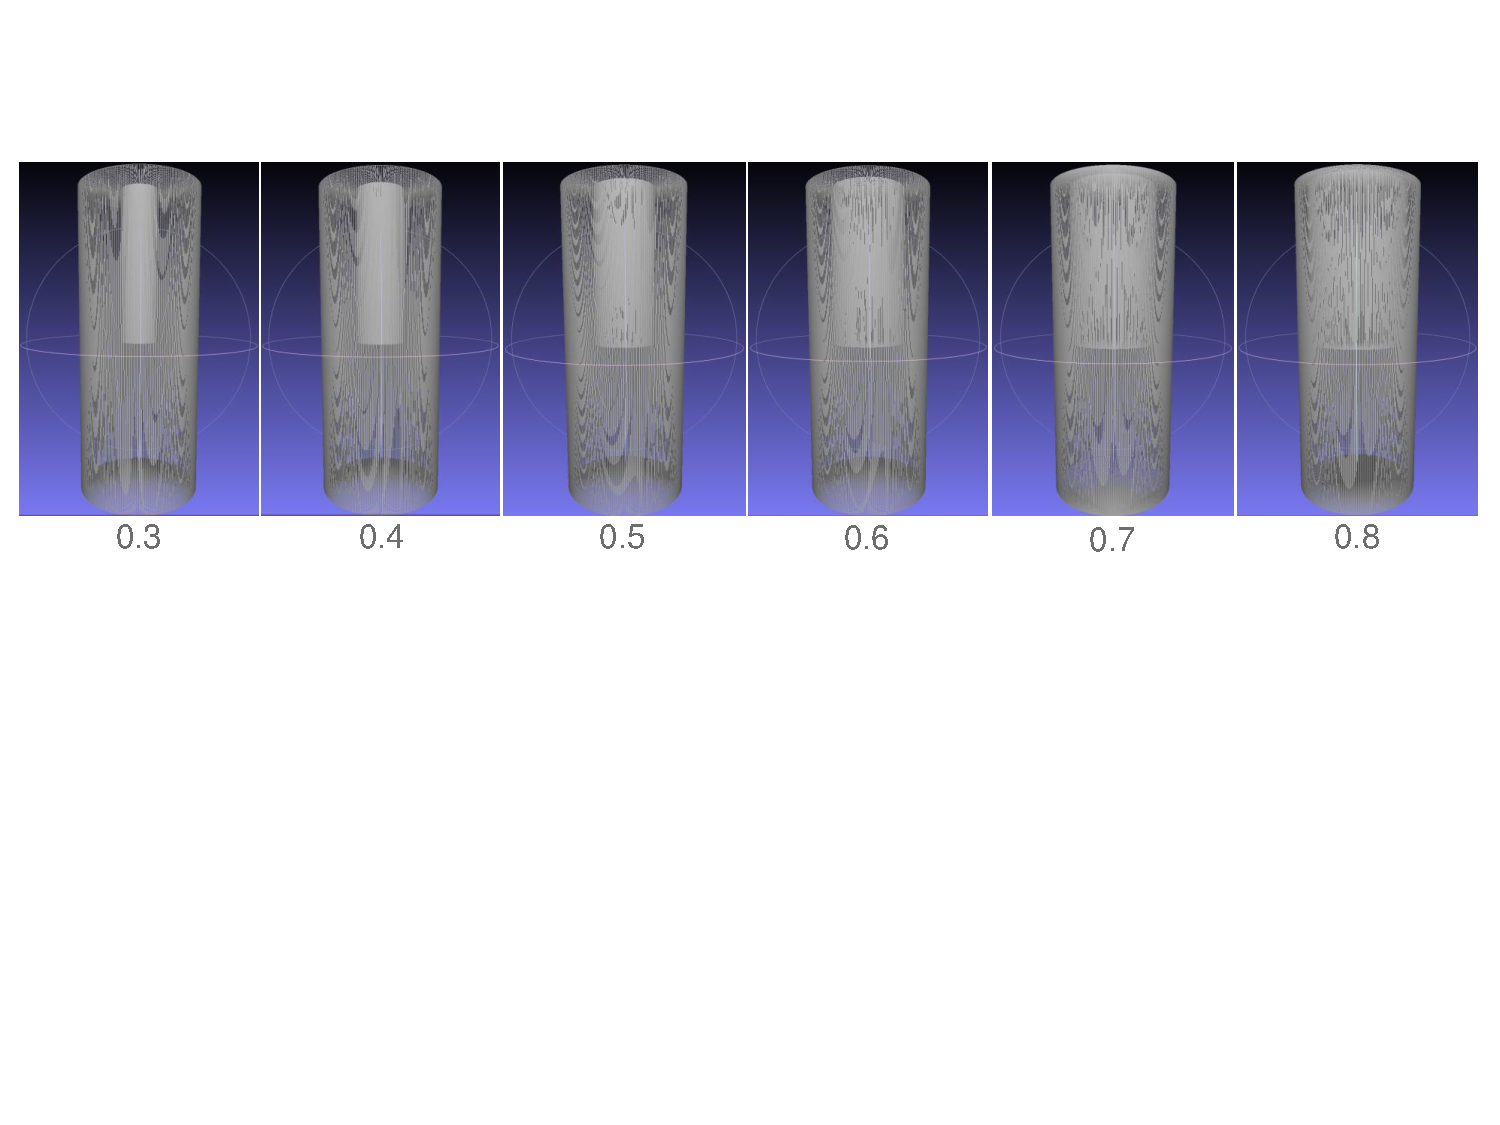
\includegraphics[width=1\linewidth]{figure/cand_inner1.pdf}}
	%\subfigure[Corresponding positional errors in green color. Brighter pixels in green indicates higher error values. ]{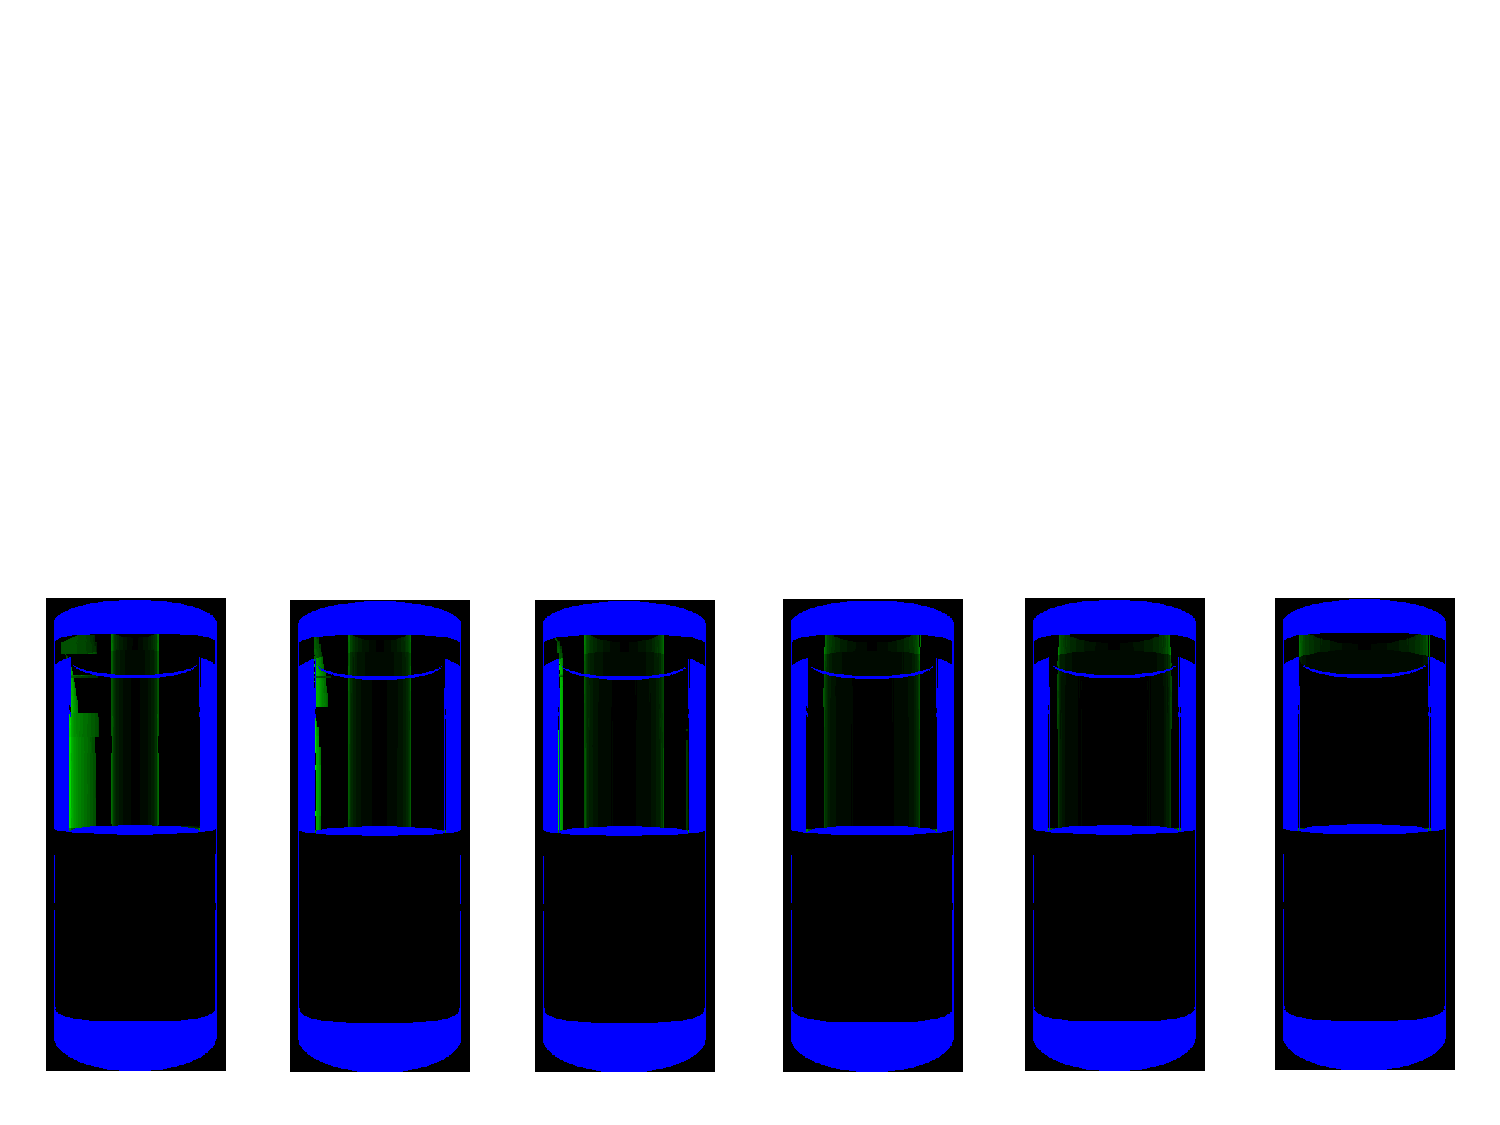
\includegraphics[width=1\linewidth]{figure/cand_inner2.pdf}}			
   %\hfill \vfill  
   %\vspace{-0.15in}
  %\caption{The variation of error map according to different inner geometry.}
%\label{cand}
%\end{figure*}

\begin{figure}
  \centering
	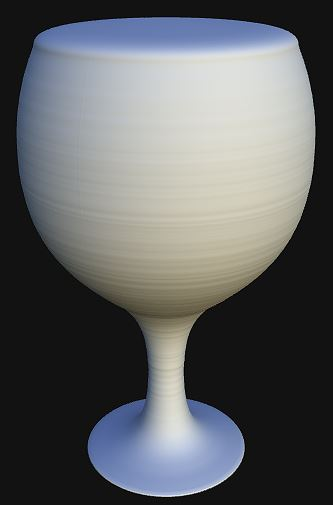
\includegraphics[height=0.7\linewidth]{figure/render_wine.JPG}	
	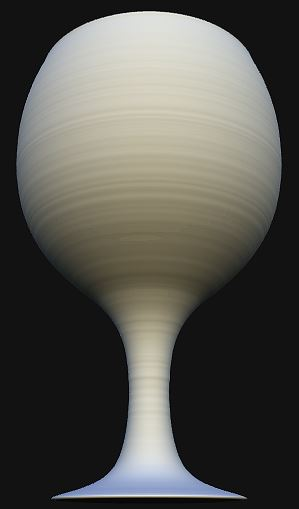
\includegraphics[height=0.7\linewidth]{figure/render_wine1.JPG}
  %\vspace{-5ex}
  \caption{A rendering result with estimated inner geometry for the target object}
  \label{render}
  %\vspace{-2ex}
\end{figure}

{\small
\bibliographystyle{ieee}
\bibliography{main}
}

\end{document}
